\documentclass[preprint, 3p,
authoryear]{elsarticle} %review=doublespace preprint=single 5p=2 column
%%% Begin My package additions %%%%%%%%%%%%%%%%%%%

\usepackage[hyphens]{url}

  \journal{Transport Geography?} % Sets Journal name

\usepackage{graphicx}
%%%%%%%%%%%%%%%% end my additions to header

\usepackage[T1]{fontenc}
\usepackage{lmodern}
\usepackage{amssymb,amsmath}
% TODO: Currently lineno needs to be loaded after amsmath because of conflict
% https://github.com/latex-lineno/lineno/issues/5
\usepackage{lineno} % add
\usepackage{ifxetex,ifluatex}
\usepackage{fixltx2e} % provides \textsubscript
% use upquote if available, for straight quotes in verbatim environments
\IfFileExists{upquote.sty}{\usepackage{upquote}}{}
\ifnum 0\ifxetex 1\fi\ifluatex 1\fi=0 % if pdftex
  \usepackage[utf8]{inputenc}
\else % if luatex or xelatex
  \usepackage{fontspec}
  \ifxetex
    \usepackage{xltxtra,xunicode}
  \fi
  \defaultfontfeatures{Mapping=tex-text,Scale=MatchLowercase}
  \newcommand{\euro}{€}
\fi
% use microtype if available
\IfFileExists{microtype.sty}{\usepackage{microtype}}{}
\usepackage[]{natbib}
\bibliographystyle{plainnat}

\usepackage{graphicx}
\ifxetex
  \usepackage[setpagesize=false, % page size defined by xetex
              unicode=false, % unicode breaks when used with xetex
              xetex]{hyperref}
\else
  \usepackage[unicode=true]{hyperref}
\fi
\hypersetup{breaklinks=true,
            bookmarks=true,
            pdfauthor={},
            pdftitle={Leveraging GTFS data to assess transit supply},
            colorlinks=false,
            urlcolor=blue,
            linkcolor=magenta,
            pdfborder={0 0 0}}

\setcounter{secnumdepth}{5}
% Pandoc toggle for numbering sections (defaults to be off)


% tightlist command for lists without linebreak
\providecommand{\tightlist}{%
  \setlength{\itemsep}{0pt}\setlength{\parskip}{0pt}}




\usepackage{booktabs}
\usepackage{longtable}
\usepackage{array}
\usepackage{multirow}
\usepackage{wrapfig}
\usepackage{float}
\usepackage{colortbl}
\usepackage{pdflscape}
\usepackage{tabu}
\usepackage{threeparttable}
\usepackage{threeparttablex}
\usepackage[normalem]{ulem}
\usepackage{makecell}
\usepackage{xcolor}



\begin{document}


\begin{frontmatter}

  \title{Leveraging GTFS data to assess transit supply}
    \author[Public Transport Research Group (PTRG)]{James Reynolds%
  \corref{cor1}%
  \fnref{1}}
   \ead{james.reynolds@monash.edu} 
    \author[Public Transport Research Group (PTRG)]{Yanda Qu%
  %
  \fnref{2}}
   \ead{yanda.qu@monash.edu} 
    \author[Public Transport Research Group (PTRG)]{Graham Currie%
  %
  \fnref{3}}
   \ead{graham.currie@monash.edu} 
      \affiliation[Public Transport Research Group (PTRG)]{
    organization={Public Transport Research Group (PTRG), Institute of
Transport Studies, Department of Civil Engineering Engineering, Monash
University},addressline={Clayton
Campus},city={Melbourne},postcode={3800},state={Victoria},country={Australia},}
    \cortext[cor1]{Corresponding author}
    \fntext[1]{Research Fellow}
    \fntext[2]{PhD Strudent}
    \fntext[2]{Professor}
  
  \begin{abstract}
  This is the abstract.

  It consists of two paragraphs.
  \end{abstract}
    \begin{keyword}
    keyword1 \sep 
    keyword2
  \end{keyword}
  
 \end{frontmatter}

\hypertarget{introduction}{%
\section{Introduction}\label{introduction}}

While ``if you can't measure it, you can't manage it'' is often
miss-attributed to \citet{Deming1993new}, who was trying to make the
opposite point \citep{Berenson2016in}, service level indicators are an
important part of researching, managing and seeking to improve transit
operations \citep{FieldingGordonJ1987Mpts, Ryus:2003aa}. A wide range of
indicators already exist including, for example: those in the Transit
Capacity and Quality of Service Manual (TCQSM)\citep{TCQSM:2013} and the
Transit Score metric \citep{WalkScore:2023tg}.

Practitioners, researchers and advocates using such metrics may face two
inter-related challenges: (1) calculating the metrics themselves for a
specific location and service pattern; and (2) explaining the metrics,
their meaning and importance to those who might not be specialists in
transit, such as to politicians or the general public. For example, the
TCQSM metrics appear difficult to calculate in practice without access
to specialist software and data. But, they appear relatively easy to
explain given they use an A to F scoring system and there is an entire
guidebook about them (although this may be offset by large number of
indicators). In contrast, Transit Scores can be obtained simply by
typing an address into a website, which will report a score out of 100
reflecting the quantity of transit available. However, Transit Scores
cannot be calculated independently as the methodolgy / algorithm is not
publicly available.

Previous research by \citet{currie2007identifying} developed a transit
Supply Index (SI) metric that appears to be both relatively easy to
calculate and relatively simple to explain to non-transport
professionals. It is obtained by calculating the number of transit
arrivals at each stop within an area of interest, with an adjustment
made to account for the typical walking distance catchment. Higher SI
scores indicate areas with higher frequency and/or better coverage.

Unfortunately, the SI does not appear to have been widely used, perhaps
in part because at the time it was first published timetable data was
not publicly available in a standardized and machine-readable format.
The scores reported in Currie and Senbergs (2007) were calculated
directly from a database of services provided by the transit authority
in Melbourne, Australia. Since then, however, the General Transit Feed
Specification (GTFS) has been developed as a way to publish timetable
data in a standardized format.\\
More than 10,000 agencies are now providing GTFS feeds\footnote{There
  are two forms: GTFS-static consisting of the timetable data (the
  scheduled services); and GTFS-realtime, which includes vehicle
  arrivals and departure times based on real-world position data. This
  paper and project uses only the GTFS-static (timetable) format.}
\citep{GTFS}, and many visulization, procession and analysis tools are
now available. A gap, however, is that there is not yet a tool to
calculate SI scores directly from a GTFS dataset. This provides the
motivation for the research reported in this paper, in which a new R
package (gtfssupplyindex) specifically developed to calculate SI scores
is presented. The remainder of this paper is structured as follows: the
next seciton outlines the background to this research, including the
original formulation of the Transit Supply Index, and an explanation of
the GTFS. Section 3 then describes the study methodology, followed by a
brief presentation of results in Section 4. Section 5 discusses the
results, outlines directions for future research and provides a
conclusion.

\hypertarget{background}{%
\section{Background}\label{background}}

\hypertarget{transit-metrics}{%
\subsection{Transit metrics}\label{transit-metrics}}

Even a brief search reveals many metrics available for benchmarking
transit services. Examples include: (1) those in the Transit Cooperative
Research Program (TCRP) Report 88, which is an extensive guidebook on
developing a performance-measurement system \citep{Ryus:2003aa}; (2)
online databases provided by the Florida Transit Information System
(FTIS) \citep{Florida-Transit-Information-System:2018aa} and
\citet{UITP:2015aa}; (3) those used in the extensive annual benchmarking
programme undertaken yearly by the Transport Strategy Centre, which
includes over 100 transit providers around the world
\citep{Imperial-College-London:2023aa}; and (4) a recently developed
methodology to calculate `blank spots' within an area, being those
places beyond 400/800 metre walking distances to/from bus and tram
stops/train stations \citep{AlamriSultan2023GAoA}.

The Fielding Triangle \citep{FieldingGordonJ1987Mpts} provides a
framework for understanding how such metrics combine service inputs,
service outputs and service consumption.\\
These can help describe cost efficiency, cost effectiveness or service
effectiveness. At a larger scale, \citet{Litman:2003ab} and
\citet{Litman:2016aa} discuss some of the traffic, mobility,
accessibility, social equity, strategic planning and other rational
decision-making frames that might underlie such transit metrics, while
\citet{Reynolds:2017ah} extends into models of how institutionalism,
incrementalism and other public policy analysis concepts might apply to
decision-making processes. Further examples include: (1)
\citet{GuzmanLuisA.2017Aeit}, who develop a measure of accessibility in
the context of policy development and social equity for Latin American
Bus Rapid Transit (BRT) networks; and (2) the street space allocation
metrics based around 10 ethical principles introduced by
\citet{Creutzig2020streetspaceallocation}.

However, many of these metrics appear difficult to calculate, complex to
explain or understand, and likely not well suited to communication with
those who are not transit planners or engineers, or other technical
specialists. Where pre-calculated metrics are immediately available it
may not be possible for practitioners, researchers or advocates to
independently generate metrics for proposed system changes. Sometimes it
is not even possible to know precisesly how scores for the existing
services levels are calculated. For example, Transit Scores for
locations with a published GTFS feed are readily available on the
\citet{WalkScore:2023tg} website, eliminating the need for any
calculations. The meaning of these Transit Scores appears easy to
explain, as the highest possible score of 100 represents what might be
experienced in the centre of New York. However, the Transit Score
algorithm is patented and effectively a black box. It is not possible to
calculate scores independently. Nor does it appear to be possible for
Transit Scores to be generated for proposed changes to networks. Transit
Score, therefore, fails the first of the aforementioned challenges, as
practitioners, researchers and advocates can only use those scores
provided online. The metric is simple to explain: the closer to 100, the
better. However, because it is based on a patented algorithm it may not
be easy to understand or explain the connection between real-world
conditions and the Transit Score, or what might need to be done to
improve the score and service levels. As such, it might partially pass
the second of the aforementioned challenges, as it is simple to
understand, yet may not withstand scrutiny.

Another example is the TCQSM, which specifies Levels of Service (LOS)
between A and F across a range of factors\footnote{ Including service
  span, frequency, speed, the proportion of the population serviced,
  competitiveness of travel times to car-based travel, and many more.}.
This scoring scheme appears relatively simple to explain\footnote{ A is
  good and F is bad. Also this scoring system matches the A to F LOS
  scoring used in many traffic capacity analysis software and manuals.},
and the detail within \citet{TCQSM:2013} provides a resource for anyone
wanting to better understand what the scores mean. However, calculation
of many of TCQSM metrics may need specialised software and
datasets\footnote{ For example, the Service Coverage Area metric in the
  TCQSM (pp.~5-8 to 5-21) may require GIS or other analysis, on top of
  accurate data about population densities, stop locations and service
  schedules.} and it might be challenging to explain the detail of these
measures or how to improve them to non-technical decision-makers,
stakeholders or others involved in transit management or advocacy.

\hypertarget{gtfs}{%
\subsection{GTFS}\label{gtfs}}

The introduction of the General Transit Feed Specification (GTFS) and
widespread release of schedule data in this format, however, has helped
towards making transit metrics more broadly available and usable. GTFS
is an open, text-based format that was developed originally to allow
transit information to be included in the Google Maps navigation
platform \citep{GTFS}.

\begin{figure}
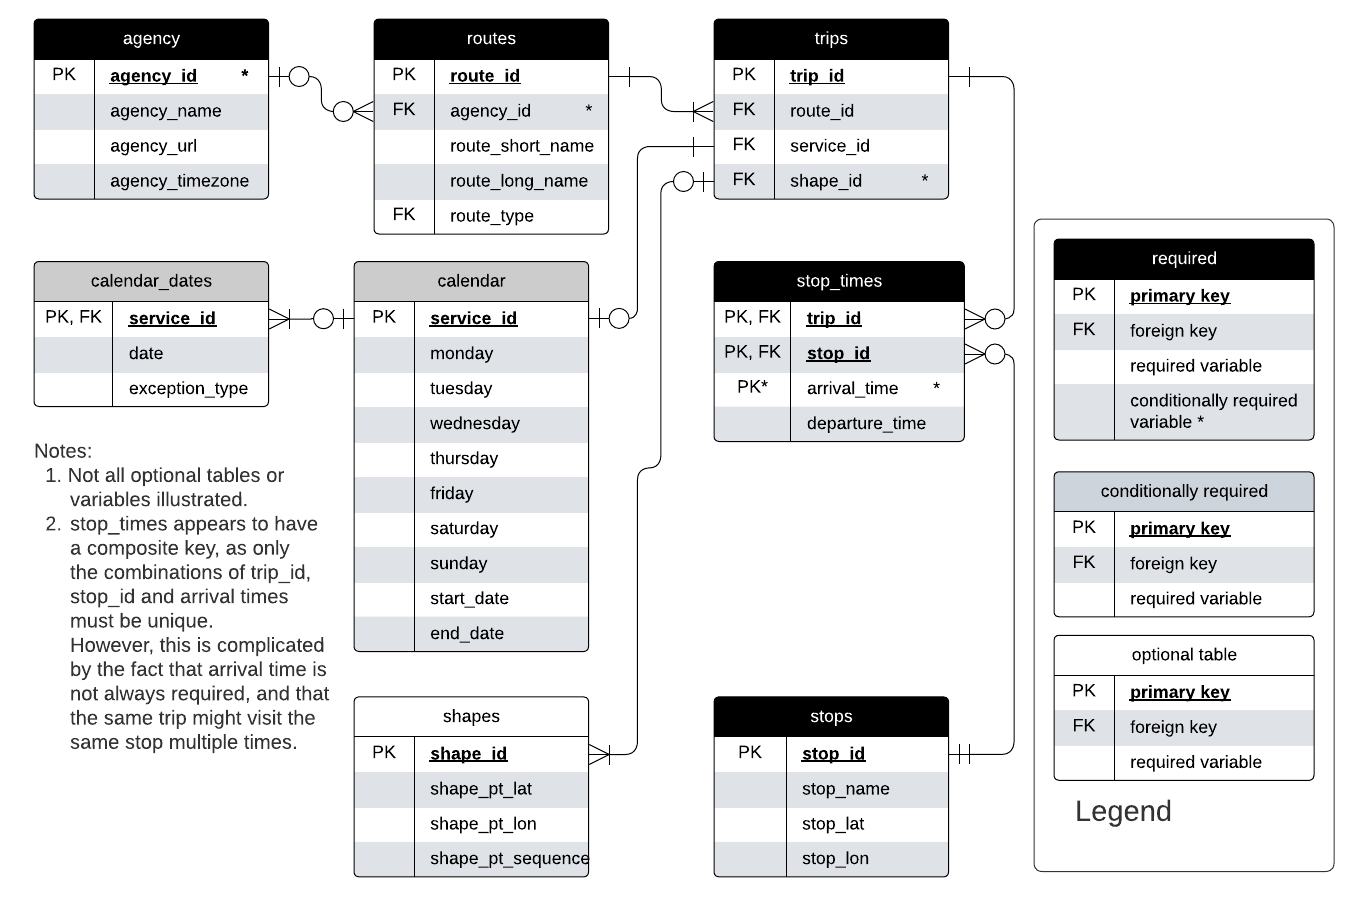
\includegraphics[width=1\linewidth]{graphics/GTFS} \caption{GTFS entity relationship diagram. Source: adapted by author from Alamri et al (2023) and the GTFS Schedule Reference (16/11/2023 revision).}\label{fig:GTFS_ERD}
\end{figure}

Figure 1 shows an Entity Relationship Diargram (ERD) of the GTFS data
structure. Each box represents a database table in the GTFS, with table
rows indicating the variables (columns) included in each\footnote{For
  example, each record in the `stops' table includes a value for
  stop\_id, stop\_name, stop\_lat and stop\_lon.}. Relationships between
the tables are indicated by the connecting lines, and Primary Key (PK)
and Foreign Key (FK) designations\footnote{For example, stop\_id also
  appears in the `stop\_times' table as a Primary Key and Foreign Key.}.
`Crow's feet' indicate the relationships between each table\footnote{See
  https://i.stack.imgur.com/fxaAq.png for guide to the symbols. But, for
  example, the stops table is required, with the stop\_id field
  providing a unique (primary) key for every stop. Within the
  stop\_times table (which is also required) the stop\_id field is a
  foreign key. Each unique stop\_id can appear many times in the
  stop\_times table, but must appear only once in the stops table. In
  the stop\_times table each combination of trip\_id, stop\_id and
  arrival time must be unique (But, see note 2!) meaning that these
  fields represent a composite key.}.

GTFS now provides a mechanism for including individual transit systems
in many online products and analyseses, including the Transit Score
metric itself. \citet{Wong:2013aa} provides another example of what can
be done with GTFS data, having developed code to calculate of some of
the TCQSM metrics\footnote{ Daily average headways, route length and
  stop numbers for 50 transit operators.}. While the \citet{Wong:2013aa}
open-source code is readily available\footnote{
  https://github.com/jcwong86/GTFS\_Explore\_Tool} this is now 11 years
old and does not appear to be currently maintained. Future research may
involve reviewing this code and using it to analyse modern GTFS feeds.
However, in this paper the aim is more modest, being to use GTFS data to
calculate Currie and Senbergs' (2007) SI.

\hypertarget{the-transit-suppy-index}{%
\subsection{The Transit Suppy Index}\label{the-transit-suppy-index}}

A generalized form of the Transit Supply Index (SI) is shown in Equation
1\footnote{Currie and Senbergs (2007) focus was the context of
  Melbourne's Census Collection Districts (CCD) and calculations based
  on a week of transit service. CCDs predate the introduction of
  Statistical Areas 1, 2, 3, and 4 (SA1, SA2, SA3, SA4), and other
  geographical divisions currently used by the Australian Bureau of
  Statistics (ABS), which may be more familiar to readers from down
  under.}.

\[SI_{area, time} = \sum{\frac{Area_{Bn}}{Area_{area}}*SL_{n, time}}\]
In Equation 1:

\begin{enumerate}
\def\labelenumi{(\arabic{enumi})}
\tightlist
\item
  \(SI_{area, time}\) is the Supply Index for the area of interest and a
  given period of time;
\item
  \(Area_{Bn}\) is the buffer area for each stop (n) within the area of
  interest. In Currie and Senbergs (2007) this was based on a radius of
  400 metres for bus and tram stops, and 800 metres for railway
  stations;
\item
  \(Area_{area}\) is the area of the area of interest; and
\item
  \(SL_{n,time}\) is the number of transit arrivals for each stop for a
  given time period.
\end{enumerate}

An advantage of the SI is that it is a relatively simple number to
calculate, understand and explain. It describes the number of transit
arrivals at stops within an area of interest and time frame, multiplied
by a factor accounting for the proportion of the area of interest that
is within typical walking distance of each stop. Hence, more services,
more stops and higher frequencies increase the score. However, the SI
does not incorporate service span, speed or other elements of a transit
service. While these may be important to passenger experience, they
might add considerable complexity. Simplicity is also helped by the way
that the SI is additive, in that \(SI_{area, time}\) scores can be
aggregated to calculate an overall score across multiple time periods or
for a region encompassing multiple areas of interest.

\hypertarget{methodology}{%
\section{Methodology}\label{methodology}}

This study involved the development of a package with tools for
calculating the SI from GTFS data. R \citep{R-base}, a widely used and
readily available statistical programming language, was adopted for code
development. The package development setup and workflow described by
\citet{wickham2023r} was adopted in this study. Various existing
packages were relied upon including: the sf package \citep{R-sf} for
geospatial analysis; the tidyverse \citep{tidyverse2019}; gtfstools
\citep{R-gtfstools}; and tidytransit \citep{R-tidytransit}. Some code
was adapted from examples, vignettes and other documentation in the
tidytransit, gtfstools and other packages.

Two cases where used as during the code development and testing so that
results might be generated for real GTFS data. These were the Mornington
Peninsula Tourist Railway GTFS feed and the Public Transport Victoria
(PTV) GTFS feed, both in Victoria, Australia. Both were selected
primarily for convenience, given that the authors are familiar with the
typical service patterns and geography. Further cases were selected as
leading, representative and contrasting examples for the results
reported here.

\hypertarget{mornington-penninsula-tourist-railway}{%
\subsection{Mornington Penninsula Tourist
Railway}\label{mornington-penninsula-tourist-railway}}

The Morning Penninsula Tourist Railway is located in the outer
south-eastern suburbs of Greater Melbourne. It runs on Sundays and
Wednesdays between Moorooduc and Mornington, with an intermediate stop
at Tanti Park\footnote{https://transitfeeds.com/p/mornington-railway/806/latest/stops}.
A GTFS feed from 2018 was selected for the purposes of tests and
demonstrating the code and output. Australian Bureau of Statistics (ABS)
data was also used, primarily through the strayr and absmapsdata
packages \citep{r-strayr}. The Mornington Peninsular Statistical Area 3
(SA3) zone and the Statistical Area 1 (SA1) zones contained within it
were adopted as the areas\_of\_interest. These are shown in Figure 1,
together with the three railway stations.

\begin{figure}
\centering
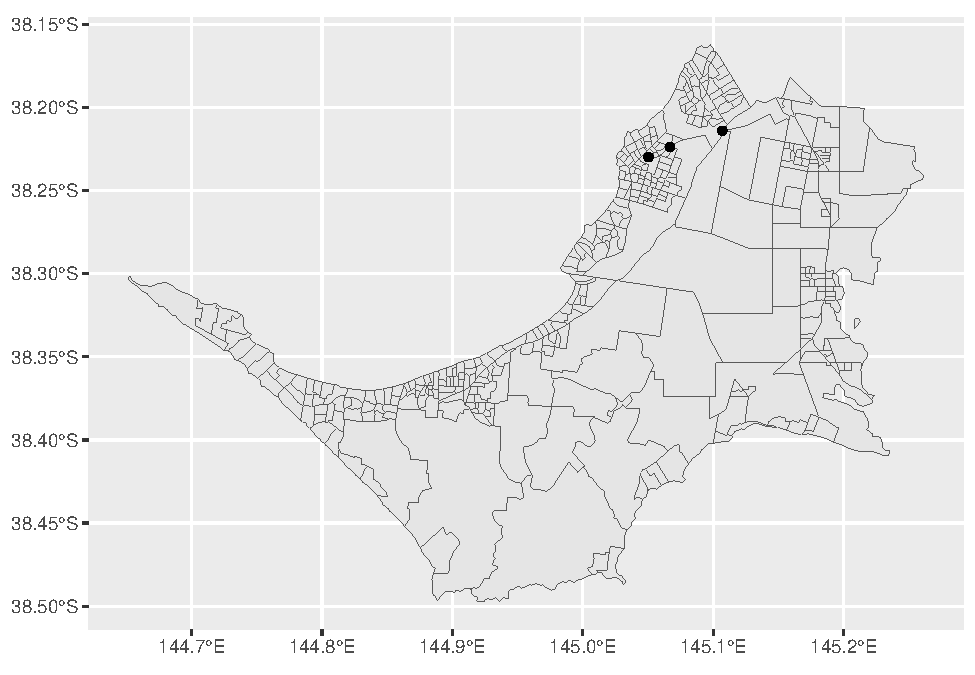
\includegraphics{Leveraging_GTFS_to_assess_transit_supply_Transport_Geography_files/figure-latex/mornington_map-1.pdf}
\caption{Mornington Penninsula SA1 zones and location of Mornington
Tourist Rail stops.}
\end{figure}

\hypertarget{public-transport-victoria-ptv}{%
\subsection{Public Transport Victoria
(PTV)}\label{public-transport-victoria-ptv}}

Larger scale testing was performed using the Victorian GTFS feed,
published by Public Transport Victoria (PTV), sourced via
\citet{transitfeeds_victoria:2023aa} for historical feeds. Again, ABS
data was used for the areas\_of\_interest.

\hypertarget{extensions}{%
\subsection{Extensions??}\label{extensions}}

Hourly ``Manhattan- and London-ised Indexes''

Tidytransit includes a sample GTFS feed from New York's MTA (including
the subway!), and so this was used for code tests were appropriate.

\hypertarget{results}{%
\section{Results}\label{results}}

\hypertarget{code-structure-and-output}{%
\subsection{Code structure and output}\label{code-structure-and-output}}

Developed code is available and documented on github
\citep{gtfssupplyindex_github}. The structure of the package and the
functions developed to generate each table are shown in Figure 2. This
indicates how the package takes input from three files: a gtfs feed
(gtfs.zip); a sf object describing the geometry of the areas for which
the SI is to be calculated; and a csv file defining the buffer zone
distances (in metres) for each route\_type\footnote{A version of this
  file is included in the package.}.

\begin{figure}
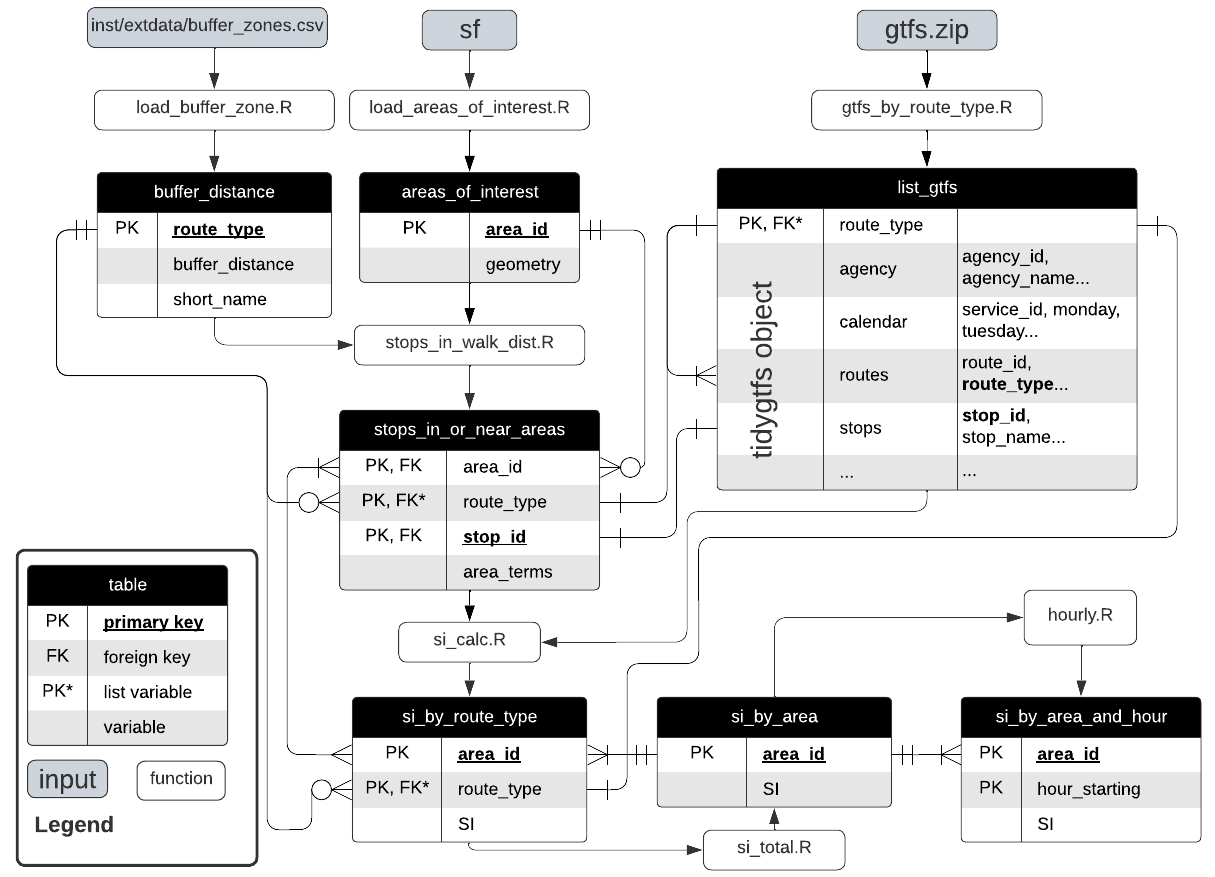
\includegraphics[width=1\linewidth]{graphics/SI_data_structure} \caption{Entity Relationship Diagram (ERD) showing the data structure and functions related to the gtfssupplyindex package}\label{fig:SI_ERD}
\end{figure}

Various data tables are output by functions included in the package. The
ultimate output (Figure 2, bottom right) is a si\_by\_area\_and\_hour
table, which reports the SI score for each hour of the day across dates
specified by the user.

\hypertarget{mornington-penninsula-results}{%
\subsection{Mornington Penninsula
results}\label{mornington-penninsula-results}}

This section shows outputs of the various functions for December 30th,
2018, for the Mornington Peninsula Tourist Railway GTFS feed. The
ultimate results, showing the SI scores for each Hourly results are
shown in Table 2.

\begin{table}

\caption{\label{tab:SI_mornington_20181230_output}Mornington Penninsula Tourist Railway hourly SI values for December 30, 2018, for SA1 zones}
\centering
\begin{tabular}[t]{l|r|r|r|r|r|r}
\hline
area\_id & 10:00 & 11:00 & 12:00 & 13:00 & 14:00 & 15:00\\
\hline
214021381 & 0.0000672 & 0.0522962 & 0.0523635 & 0.0000672 & 0.0522962 & 0.0523635\\
\hline
214021385 & 0.0000000 & 0.0067970 & 0.0067970 & 0.0000000 & 0.0067970 & 0.0067970\\
\hline
214021591 & 0.2436873 & 0.1366432 & 0.3803305 & 0.1366432 & 0.2436873 & 0.3803305\\
\hline
214021592 & 0.0684965 & 0.0000000 & 0.0684965 & 0.0000000 & 0.0684965 & 0.0684965\\
\hline
\end{tabular}
\end{table}

\begin{figure}
\centering
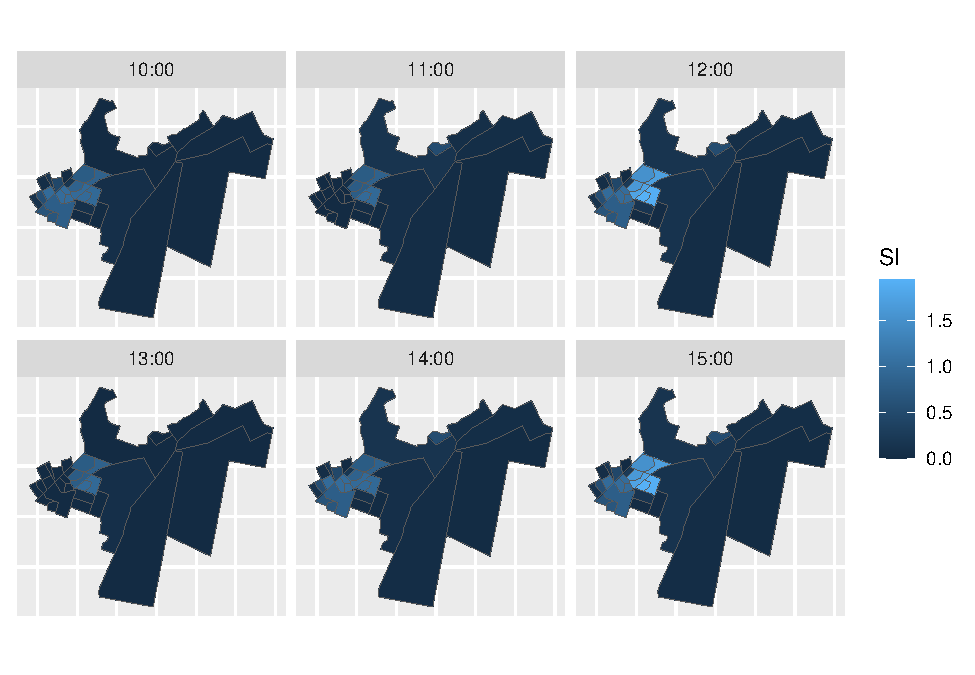
\includegraphics{Leveraging_GTFS_to_assess_transit_supply_Transport_Geography_files/figure-latex/SI_mornington_20181230_output-1.pdf}
\caption{Mornington Penninsula Tourist Railway hourly SI values for
December 30, 2018, for SA1 zones}
\end{figure}

\hypertarget{discussion-and-conclusions}{%
\section{Discussion and conclusions}\label{discussion-and-conclusions}}

\renewcommand\refname{References}
\bibliography{References.bib, packages.bib}


\end{document}
